% Preámbulo
\documentclass[stu, 12pt, letterpaper, donotrepeattitle, floatsintext, natbib]{apa7}
\usepackage[utf8]{inputenc}
\usepackage[T1]{fontenc}
\usepackage{adjustbox}
\usepackage{longtable}
\usepackage{tabularx}
\usepackage{lmodern}
\usepackage{comment}
\usepackage{marvosym}
\usepackage{graphicx}
\usepackage{float}
\usepackage[normalem]{ulem}
\usepackage[spanish]{babel}
\usepackage{multirow}
\usepackage{tabularx}
\usepackage{tabularray}
\usepackage{adjustbox}
\usepackage{geometry}
\usepackage{tikz}
\usepackage{enumitem}
\usepackage{hyperref}
\usepackage{amsmath}
\usepackage{pgfgantt}
\usepackage{apacite}
\usetikzlibrary{shapes.geometric, arrows, positioning}

\selectlanguage{spanish}
\useunder{\uline}{\ul}{}
\newcommand{\myparagraph}[1]{\paragraph{#1}\mbox{}\\}

% Portada
\title{\Large Informe de Resultados}
\author{
    Campero Morales José Antonio \\
    Campohermoso Berdeja Oscar \\
    Carrasco Cespedes Miguel Alejandro \\
    Martinez Acarapi Fabiola Alejandra \\
    Montero Garrido Diana Aneliz \\
    Zizold Sempertegui Gabriela Zulema Britta
}
\affiliation{Universidad Católica Boliviana}
\course{SIS-312: Gestión de Calidad de Sistemas}
\professor{Lic. Cecilia Alvarado Monrroy}
\duedate{\textbf{28 de octubre de 2024}}

\newcommand{\userstory}[5]{ % Change from 4 to 5 arguments
    \begin{center}
        \begin{tikzpicture}
            \node[draw, rounded corners, fill=blue!10, text width=0.9\textwidth, align=center, inner sep=10pt] {
                \textbf{#1} \\[5pt]
                \textit{Como} #2, \\[5pt]
                \textit{quiero} #3 \\[5pt]
                \textit{para} #4 \\[5pt]
                \href{#5}{Ver en GitHub} 
            };
        \end{tikzpicture}
    \end{center}
    \vspace{10pt}
}

\begin{document}
\thispagestyle{empty}

% Add the logo before the title content, avoiding extra space
\centering

\includegraphics[width=0.8\textwidth]{../imgs/logo-ucb.png} % Adjust the path to your logo image
\vspace{-5cm} % Adjust negative space if needed

\maketitle

% Índices
\newpage
\pagenumbering{roman}
% Contenido
\renewcommand\contentsname{\large Índice}
\tableofcontents
\setcounter{tocdepth}{2}
\newpage
% Fíguras
\renewcommand{\listfigurename}{\large Índice de figuras}
\listoffigures
\newpage
% Tablas
\renewcommand{\listtablename}{\large Índice de tablas}
\listoftables
\newpage

% Cuerpo
\pagenumbering{arabic}
\newpage
\section{\large Informe de Resultados}

\subsection{Resultados de los Casos de Prueba}

\noindent A continuación se documentan los resultados de los casos de prueba realizados, especificando cuáles pasaron o fallaron y detallando observaciones relevantes.

\small % Slightly reduce the font size for better fit
\renewcommand{\arraystretch}{1.0} % Slightly reduce the space between rows
\setlength{\tabcolsep}{4pt} % Reduce space between columns

\begin{longtable}{|p{2cm}|p{3cm}|p{3cm}|p{3cm}|p{3cm}|}
  \caption{Caso de prueba 1} \label{tab:casos_prueba1} \\
  \hline
    \multicolumn{5}{|l|}{\textbf{USER STORY REFERENCE: HU009-NorthWest-01, HU006-GraphEditor}} \\ \hline

  \textbf{TEST CASE ID} & \textbf{TEST DATE} & \textbf{TEST DESCRIPTION} & \textbf{TEST CONDITIONS} & \textbf{SEVERITY} \\ \hline
  \endfirsthead
  \hline
  \textbf{STEP ID} & \textbf{STEP DESCRIPTION} & \textbf{TEST DATE} & \textbf{EXPECTED RESULTS} & \textbf{ACTUAL RESULTS} \\ \hline
  \endhead
  TC1-NW & 2024-10-17 & Comprobar que, al crear los nodos y las conexiones, se genera automáticamente la matriz con los valores correctos de los pesos. & El editor debe estar configurado correctamente. Los nodos de origen y destino deben poder ser creados y conectados sin errores. Los pesos asignados deben ser valores numéricos válidos y compatibles con el sistema. & ALTA \\ \hline
\textbf{STEP ID} & \textbf{STEP DESCRIPTION} & \textbf{TEST DATE} & \textbf{EXPECTED RESULTS} & \textbf{ACTUAL RESULTS} \\ \hline
S1-1-NW & Crear 3 nodos de origen y 3 nodos de destino en el editor. & 2024-10-17 & Los 6 nodos son creados correctamente sin errores. & PASS. Los 6 nodos se crearon correctamente. \\ \hline
S2-1-NW & Asignar conexiones entre ellos con pesos específicos para cada enlace. & 2024-10-17 & Las conexiones se establecen correctamente y los pesos asignados son visibles en la interfaz. & PASS. Las conexiones inician con un peso 0, luego este valor es editable. \\ \hline
S3-1-NW & Abrir el formulario "Northwest" para ver la matriz generada. & 2024-10-17 & La matriz generada muestra los valores de los pesos correctamente, coincidiendo con los valores de las conexiones creadas. & PASS. Los valores de los pesos sean 0 o si se han editado corresponde correctamente \\ \hline
\end{longtable}
\begin{itemize}
    \item \textbf{Resumen de la Prueba:} En el Caso de Prueba 1 se verificó la creación de nodos y conexiones en el editor, y la generación automática de una matriz de pesos correcta. Todos los pasos del caso de prueba se completaron exitosamente sin errores.
    
    \item \textbf{Evaluación de la Calidad y Cumplimiento del Plan de Pruebas:} El sistema cumplió con las expectativas del plan de pruebas, mostrando los nodos y conexiones correctamente y generando una matriz de pesos precisa.
    
    \item \textbf{Desviaciones del Plan de Prueba:} No se observaron desviaciones del plan de prueba en este caso.
    
    \item \textbf{Impedimentos y Soluciones Alternativas:} No hubo impedimentos durante la ejecución de este caso de prueba.
    
    \item \textbf{Riesgos No Mitigados y Defectos No Corregidos:} No se identificaron riesgos ni defectos pendientes al finalizar esta prueba.
    
    \item \textbf{Lecciones Aprendidas y Recomendaciones:} El flujo de creación de nodos y conexiones funcionó bien, pero sería útil agregar mensajes de confirmación visuales para mejorar la experiencia del usuario.
\end{itemize}


\begin{longtable}{|p{2cm}|p{3cm}|p{3cm}|p{3cm}|p{3cm}|}
    \caption{Caso de prueba 2} \label{tab:casos_prueba2} \\
    \hline
        \multicolumn{5}{|l|}{\textbf{USER STORY REFERENCE: HU009-NorthWest-01, HU010-NorthWest-02}} \\ \hline

    \textbf{TEST CASE ID} & \textbf{TEST DATE} & \textbf{TEST DESCRIPTION} & \textbf{TEST CONDITIONS} & \textbf{SEVERITY } \\ \hline
    \endfirsthead
    \hline
    \textbf{STEP ID} & \textbf{STEP DESCRIPTION} & \textbf{TEST DATE} & \textbf{EXPECTED RESULTS} & \textbf{ACTUAL RESULTS} \\ \hline
    \endhead
    TC2-NW & 2024-10-17 & Verificar el comportamiento del sistema cuando la suma de la oferta y la demanda no es igual. & El editor debe estar configurado correctamente. Los nodos de origen y destino deben poder ser creados y conectados sin errores. Los pesos asignados deben ser valores numéricos válidos y compatibles con El sistema. La oferta total debe ser mayor que  la demanda. & MEDIA                                                                                                     \\ \\ \hline
    \textbf{STEP ID} & \textbf{STEP DESCRIPTION} & \textbf{TEST DATE} & \textbf{EXPECTED RESULTS} & \textbf{ACTUAL RESULTS} \\ \hline
    S1-2-NW & Ingresar 100 unidades de oferta para los nodos de origen & 2024-10-17 & El sistema debe aceptar la cantidad de oferta sin mostrar errores. & PASS. Se muestra la cantidad de ofertta sin mostrar errores. \\ \hline
    S2-2-NW & Ingresar 80 unidades de demanda para los nodos de destino. & 2024-10-17 & El sistema debe aceptar la cantidad de demanda sin mostrar errores. & PASS. La cantidad de demanda se muestra sin errores. \\ \hline
    S3-2-NW & Ejecutar el cálculo utilizando el método de la esquina noroeste. & 2024-10-17 & El sistema debe detectar que la oferta y la demanda no están balanceadas y ajustar automáticamente la solución (por ejemplo, añadiendo un nodo ficticio) para resolver el problema de transporte sin errores. & FAIL. El sistema no detecta que la oferta y la demanda no están balanceados, y no se ajusta la solución. \\ \hline
\end{longtable}

\begin{itemize}
    \item \textbf{Resumen de la Prueba:} Este caso de prueba verificó el comportamiento del sistema cuando la oferta y demanda no estaban balanceadas. Se identificó un fallo en el ajuste automático cuando estos valores no coincidían.
    
    \item \textbf{Evaluación de la Calidad y Cumplimiento del Plan de Pruebas:} El sistema no cumplió con el comportamiento esperado, ya que no detectó el desbalance y no ajustó la solución automáticamente.
    
    \item \textbf{Desviaciones del Plan de Prueba:} Se observó una desviación en cuanto al comportamiento del sistema al no ajustar la oferta y demanda desbalanceadas.
    
    \item \textbf{Impedimentos y Soluciones Alternativas:} No hubo impedimentos adicionales; sin embargo, se sugiere implementar una alerta o ajuste automático para estos escenarios.
    
    \item \textbf{Riesgos No Mitigados y Defectos No Corregidos:} El sistema presenta un riesgo de error en la optimización en escenarios de desbalance entre oferta y demanda.
    \item \textbf{Lecciones Aprendidas y Recomendaciones:} Se recomienda mejorar la validación del balance entre oferta y demanda, implementando un nodo ficticio automático para evitar problemas en la solución
\end{itemize}



\begin{longtable}{|p{2cm}|p{3cm}|p{3cm}|p{3cm}|p{3cm}|}
    \caption{Caso de prueba 3} \label{tab:casos_prueba3} \\
    \hline
        \multicolumn{5}{|l|}{\textbf{USER STORY REFERENCE: HU010-NorthWest-02, HU010-NorthWest-03}} \\ \hline

    \textbf{TEST CASE ID} & \textbf{TEST DATE} & \textbf{TEST DESCRIPTION} & \textbf{TEST CONDITIONS} & \textbf{SEVERITY } \\ \hline
    \endfirsthead
    \hline
    \textbf{STEP ID} & \textbf{STEP DESCRIPTION} & \textbf{TEST DATE} & \textbf{EXPECTED RESULTS} & \textbf{ACTUAL RESULTS} \\ \hline
    \endhead
    TC3-NW & 2024-10-17 & Verificar que las opciones de maximizar y minimizar generen soluciones distintas. & El editor debe estar configurado correctamente, permitiendo crear y conectar nodos. Pesos numéricos válidos y matriz de costos conocida. & ALTA \\ \hline
    \textbf{STEP ID} & \textbf{STEP DESCRIPTION} & \textbf{TEST DATE} & \textbf{EXPECTED RESULTS} & \textbf{ACTUAL RESULTS} \\ \hline
    S1-3-NW & Configurar la matriz de costos. & 2024-10-17 & El sistema acepta la matriz de costos sin errores y la muestra correctamente. & PASS. Matriz aceptada y mostrada correctamente. \\ \hline
    S2-3-NW & Seleccionar maximización y calcular. & 2024-10-17 & El sistema calcula y muestra la solución sin errores. & PASS. Calcula solución sin errores pero no alerta sobre datos problemáticos. \\ \hline
    S3-3-NW & Verificar la solución en maximización. & 2024-10-17 & Solución visible y accesible en la interfaz. & PASS. Solución visible y accesible. \\ \hline
    S4-3-NW & Seleccionar minimización y calcular. & 2024-10-17 & El sistema calcula y muestra la solución sin errores. & PASS. Calcula correctamente en minimización. \\ \hline
    S5-3-NW & Comparar ambas soluciones. & 2024-10-17 & Las soluciones deben diferir según el criterio de optimización. & PASS. Solución máxima y mínima obtenidas. \\ \hline
\end{longtable}
\begin{itemize}
    \item \textbf{Resumen de la Prueba:} Se probó que el sistema generara diferentes soluciones de maximización y minimización. El sistema logró calcular ambas soluciones correctamente.
    
    \item \textbf{Evaluación de la Calidad y Cumplimiento del Plan de Pruebas:} La prueba cumplió con los estándares de calidad, generando soluciones distintas para los criterios de maximización y minimización.
    
    \item \textbf{Desviaciones del Plan de Prueba:} No hubo desviaciones en este caso de prueba.
    
    \item \textbf{Impedimentos y Soluciones Alternativas:} No se identificaron impedimentos para la ejecución de esta prueba.
    
    \item \textbf{Riesgos No Mitigados y Defectos No Corregidos:} No se identificaron riesgos ni defectos pendientes en esta prueba.
    
    \item \textbf{Lecciones Aprendidas y Recomendaciones:} Se recomienda incluir una verificación automática que confirme la diferencia entre las soluciones de maximización y minimización para facilitar la validación.
\end{itemize}

\begin{longtable}{|p{2cm}|p{3cm}|p{3cm}|p{3cm}|p{3cm}|}
    \caption{Caso de prueba 4} \label{tab:casos_prueba4} \\
    \hline
        \multicolumn{5}{|l|}{\textbf{USER STORY REFERENCE: HU009-NorthWest-01, HU010-NorthWest-03}} \\ \hline

    \textbf{TEST CASE ID} & \textbf{TEST DATE} & \textbf{TEST DESCRIPTION} & \textbf{TEST CONDITIONS} & \textbf{SEVERITY} \\ \hline

    \endfirsthead
    \hline
    \textbf{STEP ID} & \textbf{STEP DESCRIPTION} & \textbf{TEST DATE} & \textbf{EXPECTED RESULTS} & \textbf{ACTUAL RESULTS} \\ \hline
    \endhead
    TC4-NW & 2024-10-17 & Verificar que el sistema siempre genere una solución factible para diferentes configuraciones de oferta y demanda. & El editor debe estar configurado correctamente. Los nodos de origen y destino deben poder ser creados y conectados sin errores. Los pesos asignados deben ser valores numéricos válidos y compatibles con El sistema. Varias configuraciones de oferta y demanda, incluyendo configuraciones balanceadas y no balanceadas. & ALTA                                                                                           \\ \\ \hline
    \textbf{STEP ID} & \textbf{STEP DESCRIPTION} & \textbf{TEST DATE} & \textbf{EXPECTED RESULTS} & \textbf{ACTUAL RESULTS} \\ \hline
    S1-4-NW & Ingresar diferentes valores de oferta y demanda (balanceados y no balanceados). & 2024-10-17 & El sistema debe aceptar los valores de oferta y demanda sin errores, independientemente de si están balanceados. & PASS. Si acepta cualquier tipo de valores sin ningún error. \\ \hline
    S2-4-NW & Ejecutar el cálculo del problema de transporte utilizando el módulo "Northwest". & 2024-10-17 & El sistema debe generar una solución válida y consistente, sin importar si la configuración de oferta y demanda está balanceada. & FAIL. Si genera soluciones, aunque no siempre es valida \\ \hline
\end{longtable}
\begin{itemize}
    \item \textbf{Resumen de la Prueba:} El objetivo de este caso fue verificar que el sistema generara una solución factible en diferentes configuraciones de oferta y demanda. Hubo un fallo al intentar generar soluciones válidas en configuraciones no balanceadas.
    
    \item \textbf{Evaluación de la Calidad y Cumplimiento del Plan de Pruebas:} El sistema falló en cumplir con los requisitos del plan de pruebas, ya que no siempre generó una solución válida en configuraciones no balanceadas.
    
    \item \textbf{Desviaciones del Plan de Prueba:} Se observó que el sistema no pudo adaptarse adecuadamente en configuraciones no balanceadas.
    
    \item \textbf{Impedimentos y Soluciones Alternativas:} No hubo impedimentos adicionales, pero se sugiere una revisión del algoritmo para mejorar la estabilidad en casos de desbalance.
    
    \item \textbf{Riesgos No Mitigados y Defectos No Corregidos:} Existe el riesgo de obtener resultados inconsistentes en configuraciones no balanceadas, lo cual puede impactar la precisión del sistema.
    
    \item \textbf{Lecciones Aprendidas y Recomendaciones:} Es recomendable implementar una validación para alertar al usuario en configuraciones de oferta y demanda no balanceadas y evitar errores.
\end{itemize}

\begin{longtable}{|p{2cm}|p{3cm}|p{3cm}|p{3cm}|p{3cm}|}
    \caption{Caso de prueba 5} \label{tab:casos_prueba5} \\
    \hline
        \multicolumn{5}{|l|}{\textbf{USER STORY REFERENCE: HU009-NorthWest-02}} \\ \hline

    \textbf{TEST CASE ID} & \textbf{TEST DATE} & \textbf{TEST DESCRIPTION} & \textbf{TEST CONDITIONS} & \textbf{SEVERITY} \\ \hline
    \endfirsthead
    \hline
    \textbf{STEP ID} & \textbf{STEP DESCRIPTION} & \textbf{TEST DATE} & \textbf{EXPECTED RESULTS} & \textbf{ACTUAL RESULTS} \\ \hline
    \endhead
    TC5-NW & 2024-10-17 & Asegurarse de que el formulario de entrada de datos sea intuitivo y que los campos obligatorios estén correctamente validados. & El editor debe estar configurado correctamente. Los nodos de origen y destino deben poder ser creados y conectados sin errores. Datos válidos e inválidos en el formulario de entrada, incluyendo campos vacíos y datos no numéricos en los campos de oferta y demanda. & ALTA \\ \hline
    \textbf{STEP ID} & \textbf{STEP DESCRIPTION} & \textbf{TEST DATE} & \textbf{EXPECTED RESULTS} & \textbf{ACTUAL RESULTS} \\ \hline
    S1-5-NW & Intentar enviar el formulario con algunos campos vacíos. & 2024-10-17 & El sistema debe mostrar mensajes de error específicos indicando que los campos obligatorios están vacíos. & FAIL. El sistema no muestra mensajes de error específicos ni indica que los campos son obligatorios. \\ \hline
    S2-5-NW & Ingresar datos no numéricos en los campos de oferta y demanda y enviar el formulario. & 2024-10-17 & El sistema debe mostrar mensajes de error indicando que los valores en oferta y demanda deben ser numéricos. & FAIL. El sistema no muestra mensajes de error ni indica que los valores necesiten ser numéricos. \\ \hline
    S3-5-NW & Ingresar datos válidos en todos los campos y enviar el formulario, sin demanda y oferta. & 2024-10-17 & El sistema debe lanzar un mensaje de error porque los datos de demanda y oferta deberían ser obligatorios. & FAIL. El sistema permite enviar los datos, pero no muestra error cuando los datos obligatorios de demanda y oferta están vacíos. \\ \hline
\end{longtable}
\begin{itemize}
    \item \textbf{Resumen de la Prueba:} Se evaluó la usabilidad del formulario de entrada de datos, incluyendo la validación de campos obligatorios. Se identificaron fallos en la validación de campos vacíos y no numéricos.
    
    \item \textbf{Evaluación de la Calidad y Cumplimiento del Plan de Pruebas:} El sistema no cumplió con los requisitos de usabilidad esperados, al permitir el envío de datos inválidos sin mostrar mensajes de error.
    
    \item \textbf{Desviaciones del Plan de Prueba:} La ausencia de validación en campos obligatorios representó una desviación significativa del plan de pruebas.
    
    \item \textbf{Impedimentos y Soluciones Alternativas:} No hubo impedimentos, pero se sugiere implementar validaciones adicionales en los campos del formulario.
    
    \item \textbf{Riesgos No Mitigados y Defectos No Corregidos:} El sistema presenta riesgos de errores de entrada al no validar adecuadamente los campos obligatorios.
    
    \item \textbf{Lecciones Aprendidas y Recomendaciones:} Es esencial fortalecer la validación de datos en el formulario para mejorar la experiencia y prevenir errores de entrada.
\end{itemize}
\small % Slightly reduce the font size for better fit
\renewcommand{\arraystretch}{1.0} % Slightly reduce the space between rows
\setlength{\tabcolsep}{4pt} % Reduce space between columns

\begin{longtable}{|p{2cm}|p{3cm}|p{3cm}|p{3cm}|p{3cm}|}
    \caption{Caso de prueba 6} \label{tab:casos_prueba6} \\
    \hline
        \multicolumn{5}{|l|}{\textbf{USER STORY REFERENCE: HU006-GraphEditor}} \\ \hline

    \textbf{TEST CASE ID} & \textbf{TEST DATE} & \textbf{TEST DESCRIPTION} & \textbf{TEST CONDITIONS} & \textbf{SEVERITY} \\ \hline
    \endfirsthead
    \hline
    \textbf{STEP ID} & \textbf{STEP DESCRIPTION} & \textbf{TEST DATE} & \textbf{EXPECTED RESULTS} & \textbf{ACTUAL RESULTS} \\ \hline
    \endhead
    TC6-NW & 2024-10-17 & Verificar que el editor permita a los usuarios definir nodos y conexiones con pesos, y que los grafos se visualicen de forma intuitiva en la interfaz. & Configuración inicial del editor sin grafos; usuarios con capacidad de definir nodos y conexiones. & ALTA \\ \hline
    \textbf{STEP ID} & \textbf{STEP DESCRIPTION} & \textbf{TEST DATE} & \textbf{EXPECTED RESULTS} & \textbf{ACTUAL RESULTS} \\ \hline
    S1-6-NW & Definir un nodo en el editor. & 2024-10-17 & El nodo debe aparecer inmediatamente en la visualización gráfica del editor. & PASS. El nodo aparece de manera inmediata en la visualización en el editor. \\ \hline
    S2-6-NW & Ingresar datos válidos en todos los campos y enviar el formulario. & 2024-10-17 & La conexión debe visualizarse en el grafo en tiempo real, mostrando el peso asignado. & PASS. La conexión se visualiza en tiempo real y asigna un peso 0. \\ \hline
    S3-6-NW & Intentar crear una conexión con datos inconsistentes (por ejemplo, un peso no numérico). & 2024-10-17 & El sistema debe notificar al usuario sobre la inconsistencia en la entrada de datos, previniendo errores en la creación del grafo. & FAIL. El sistema evita la inconsistencia de los datos, pero no notifica sobre errores. \\ \hline
    S4-6-NW & Modificar la conexión o el nodo existente. & 2024-10-17 & La visualización del grafo debe actualizarse de inmediato para reflejar los cambios realizados. & PASS. Los cambios al grafo se producen de manera inmediata. \\ \hline
\end{longtable}
\begin{itemize}
    \item \textbf{Resumen de la Prueba:} Este caso de prueba se centró en la creación y visualización de grafos en el editor. El sistema logró representar correctamente los nodos y conexiones, pero falló al manejar datos inconsistentes sin notificar al usuario.
    
    \item \textbf{Evaluación de la Calidad y Cumplimiento del Plan de Pruebas:} El sistema cumplió parcialmente con el plan de pruebas, aunque falló en la notificación de errores para datos inconsistentes.
    
    \item \textbf{Desviaciones del Plan de Prueba:} No se detectaron desviaciones mayores, salvo la falta de notificación en entradas inconsistentes.
    
    \item \textbf{Impedimentos y Soluciones Alternativas:} No hubo impedimentos, pero se sugiere implementar notificaciones para datos inválidos en el editor.
    
    \item \textbf{Riesgos No Mitigados y Defectos No Corregidos:} El riesgo de errores sin notificación puede llevar a confusión en el usuario al ingresar datos incorrectos.
    
    \item \textbf{Lecciones Aprendidas y Recomendaciones:} Se recomienda mejorar las notificaciones de error para que el usuario esté informado de inconsistencias de entrada.
\end{itemize}

\small % Slightly reduce the font size for better fit
\renewcommand{\arraystretch}{1.0} % Slightly reduce the space between rows
\setlength{\tabcolsep}{4pt} % Reduce space between columns

\begin{longtable}{|p{2cm}|p{3cm}|p{3cm}|p{3cm}|p{3cm}|}
    \caption{Caso de prueba 7} \label{tab:casos_prueba7} \\
    \hline
        \multicolumn{5}{|l|}{\textbf{USER STORY REFERENCE: HU008-FileManagement}} \\ \hline

    \textbf{TEST CASE ID} & \textbf{TEST DATE} & \textbf{TEST DESCRIPTION} & \textbf{TEST CONDITIONS} & \textbf{SEVERITY} \\ \hline
    \endfirsthead
    \hline
    \textbf{STEP ID} & \textbf{STEP DESCRIPTION} & \textbf{TEST DATE} & \textbf{EXPECTED RESULTS} & \textbf{ACTUAL RESULTS} \\ \hline
    \endhead
    TC7-NW & 2024-10-17 & Verificar que el editor permita cargar grafos desde el computador en formato JSON y descargar los grafos creados, con notificaciones de éxito o error en las operaciones. & Grafo guardado en formato JSON en el computador; editor configurado para cargar y descargar grafos. & ALTA \\ \hline
    \textbf{STEP ID} & \textbf{STEP DESCRIPTION} & \textbf{TEST DATE} & \textbf{EXPECTED RESULTS} & \textbf{ACTUAL RESULTS} \\ \hline
    S1-7-NW & Cargar un archivo JSON de grafo desde el computador al editor. & 2024-10-17 & El grafo debe aparecer correctamente en el editor, conservando todos los nodos y conexiones, y el sistema debe notificar que la carga fue exitosa. & PASS. El grafo aparece correctamente en el editor, y conserva todos los nodos y conexiones. \\ \hline
    S2-7-NW & Intentar cargar un archivo JSON con datos incompletos o en formato incorrecto. & 2024-10-17 & El sistema debe mostrar un mensaje de error indicando el problema con el archivo, sin cargar datos incompletos en el editor. & FAIL. El sistema no muestra ningún mensaje de error. \\ \hline
    S3-7-NW & Descargar el grafo actualmente visualizado en el editor en formato JSON. & 2024-10-17 & El archivo debe descargarse correctamente, conservando toda la información de nodos y conexiones, y el sistema debe notificar que la descarga fue exitosa. & PASS. El archivo se descarga correctamente con toda la información, y el sistema notifica que la descarga fue exitosa. \\ \hline
\end{longtable}
\begin{itemize}
    \item \textbf{Resumen de la Prueba:} Este caso evaluó la funcionalidad de carga y descarga de grafos en formato JSON. Hubo éxito en la mayoría de las pruebas, pero fallos al cargar archivos en formato incorrecto sin notificación de error.
    
    \item \textbf{Evaluación de la Calidad y Cumplimiento del Plan de Pruebas:} El sistema logró cargar y descargar archivos correctamente, pero no cumplió con el estándar de calidad al no notificar errores en archivos incorrectos.
    
    \item \textbf{Desviaciones del Plan de Prueba:} Se identificó una desviación en la falta de notificación de errores al cargar archivos en formato incorrecto.
    
    \item \textbf{Impedimentos y Soluciones Alternativas:} No hubo impedimentos, aunque se sugiere mejorar la detección y notificación de errores de carga.
    
    \item \textbf{Riesgos No Mitigados y Defectos No Corregidos:} La falta de notificación de errores al cargar archivos defectuosos representa un riesgo para la integridad de los datos cargados.
    
    \item \textbf{Lecciones Aprendidas y Recomendaciones:} Es importante implementar mensajes de error específicos para archivos en formato incorrecto, mejorando la usabilidad del sistema.
\end{itemize}

\section{Reporte y Resultados}

\subsection{Reporte de Defectos}

\noindent Se identificaron los siguientes defectos (bugs) durante la ejecución de los casos de prueba:

\begin{longtable}{|p{5cm}|p{10cm}|}
    \caption{Reporte de Defecto TC2-NW} \label{tab:reporte_defecto_tc2} \\
    \hline
    \textbf{Test Case Reference} & TC2-NW \\ \hline
    \textbf{ID} & DEF-001 \\ \hline
    \textbf{Title} & Falta de ajuste automático en desbalance de oferta y demanda \\ \hline
    \textbf{Description} & El sistema no ajusta automáticamente la solución cuando la oferta y demanda están desbalanceadas, impidiendo resolver correctamente el problema de transporte. \\ \hline
    \textbf{Steps to Reproduce} & 
    1. Ingresar 100 unidades de oferta para los nodos de origen. \newline
    2. Ingresar 80 unidades de demanda para los nodos de destino. \newline
    3. Ejecutar el cálculo utilizando el método de la esquina noroeste. \\ \hline
    \textbf{Expected Result} & El sistema debe detectar que la oferta y la demanda no están balanceadas y ajustar automáticamente la solución (por ejemplo, añadiendo un nodo ficticio) para resolver el problema de transporte sin errores. \\ \hline
    \textbf{Actual Result} & FAIL. El sistema no detecta que la oferta y la demanda no están balanceados, y no se ajusta la solución. \\ \hline
    \textbf{Evidence} & \url{https://drive.google.com/drive/folders/1YT13XV8GKL1_5Vs0Eiqv073T4WOpTW_h?usp=drive_link} \\ \hline
    \textbf{Severity} & Alta \\ \hline
    \textbf{Priority} & Alta \\ \hline
\end{longtable}

\begin{longtable}{|p{5cm}|p{10cm}|}
    \caption{Reporte de Defecto TC4-NW} \label{tab:reporte_defecto_tc4} \\
    \hline
    \textbf{Test Case Reference} & TC4-NW \\ \hline
    \textbf{ID} & DEF-002 \\ \hline
    \textbf{Title} & Generación de soluciones no válidas en configuraciones desbalanceadas \\ \hline
    \textbf{Description} & El sistema genera soluciones inconsistentes cuando la configuración de oferta y demanda no está balanceada, afectando la precisión de los resultados. \\ \hline
    \textbf{Steps to Reproduce} & 
    1. Ingresar diferentes valores de oferta y demanda (balanceados y no balanceados). \newline
    2. Ejecutar el cálculo del problema de transporte utilizando el módulo "Northwest". \\ \hline
    \textbf{Expected Result} & El sistema debe generar una solución válida y consistente, sin importar si la configuración de oferta y demanda está balanceada. \\ \hline
    \textbf{Actual Result} & FAIL. Si genera soluciones, aunque no siempre es válida. \\ \hline
    \textbf{Evidence} & \url{https://drive.google.com/drive/folders/17rGON0-rO-N2L-eLUU5vKIduLq4BL2vu?usp=drive_link} \\ \hline
    \textbf{Severity} & Alta \\ \hline
    \textbf{Priority} & Alta \\ \hline
\end{longtable}

\begin{longtable}{|p{5cm}|p{10cm}|}
    \caption{Reporte de Defecto TC5-NW} \label{tab:reporte_defecto_tc5} \\
    \hline
    \textbf{Test Case Reference} & TC5-NW \\ \hline
    \textbf{ID} & DEF-003 \\ \hline
    \textbf{Title} & Falta de validación y mensajes de error en campos obligatorios y numéricos \\ \hline
    \textbf{Description} & El sistema permite el envío de datos sin validar campos obligatorios ni valores numéricos, y no muestra mensajes de error en campos incorrectos o vacíos. \\ \hline
    \textbf{Steps to Reproduce} & 
    1. Intentar enviar el formulario con algunos campos vacíos. \newline
    2. Ingresar datos no numéricos en los campos de oferta y demanda y enviar el formulario. \newline
    3. Ingresar datos válidos en todos los campos y enviar el formulario, sin demanda y oferta. \\ \hline
    \textbf{Expected Result} & El sistema debe mostrar mensajes de error específicos indicando que los campos obligatorios están vacíos, que los valores en oferta y demanda deben ser numéricos, y que estos datos deben ser obligatorios. \\ \hline
    \textbf{Actual Result} & FAIL. El sistema no muestra mensajes de error específicos ni indica que los campos son obligatorios o que deben ser numéricos. \\ \hline
    \textbf{Evidence} & \url{https://drive.google.com/drive/folders/10bwq9Ha9stscJcG6weDrUWH_h_Sp8eGR?usp=drive_link} \\ \hline
    \textbf{Severity} & Alta \\ \hline
    \textbf{Priority} & Alta \\ \hline
\end{longtable}

\begin{longtable}{|p{5cm}|p{10cm}|}
    \caption{Reporte de Defecto TC6-NW} \label{tab:reporte_defecto_tc6} \\
    \hline
    \textbf{Test Case Reference} & TC6-NW \\ \hline
    \textbf{ID} & DEF-004 \\ \hline
    \textbf{Title} & Falta de notificación de inconsistencias en datos al crear conexiones \\ \hline
    \textbf{Description} & El sistema permite crear conexiones con datos inconsistentes sin notificar al usuario sobre los errores en los datos ingresados. \\ \hline
    \textbf{Steps to Reproduce} & 
    1. Definir un nodo en el editor. \newline
    2. Ingresar datos válidos en todos los campos y enviar el formulario. \newline
    3. Intentar crear una conexión con datos inconsistentes (por ejemplo, un peso no numérico). \\ \hline
    \textbf{Expected Result} & El sistema debe notificar al usuario sobre la inconsistencia en la entrada de datos, previniendo errores en la creación del grafo. \\ \hline
    \textbf{Actual Result} & FAIL. El sistema evita la inconsistencia de los datos pero no notifica sobre errores. \\ \hline
    \textbf{Evidence} & \url{https://drive.google.com/drive/folders/1uA5hSTQQ20aGa1zVK830kfKvrHaQ8wZS?usp=drive_link} \\ \hline
    \textbf{Severity} & Media \\ \hline
    \textbf{Priority} & Media \\ \hline
\end{longtable}

\begin{longtable}{|p{5cm}|p{10cm}|}
    \caption{Reporte de Defecto TC1-NW} \label{tab:reporte_defecto_tc1} \\
    \hline
    \textbf{Test Case Reference} & TC1-NW \\ \hline
    \textbf{ID} & DEF-005 \\ \hline
    \textbf{Title} & Bloqueo del editor al modificar el grafo tras ejecutar el algoritmo \\ \hline
    \textbf{Description} & Después de ejecutar el algoritmo de la esquina noroeste, el editor se bloquea, impidiendo realizar modificaciones en el grafo. Solo vuelve a funcionar después de presionar Enter. \\ \hline
    \textbf{Steps to Reproduce} & 
    1. Solicitar la solución utilizando el método Northwest. \newline
    2. Intentar volver al editor para hacer modificaciones en el grafo. \\ \hline
    \textbf{Expected Result} & Después de ejecutar el algoritmo, el editor debe permitir al usuario modificar el grafo sin problemas. \\ \hline
    \textbf{Actual Result} & El editor se bloquea y no permite realizar ninguna acción. Solo vuelve a funcionar al presionar Enter. \\ \hline
    \textbf{Evidence} & \url{https://drive.google.com/drive/folders/1VqBzMIqzObjwQ7AbNkVM1nD7D_-MKnde?usp=drive_link} \\ \hline
    \textbf{Severity} & Alta \\ \hline
    \textbf{Priority} & Alta \\ \hline
\end{longtable}


\subsection{Resultados de las Métricas del Plan de Pruebas}

\noindent A continuación, se presentan las métricas recopiladas:

\begin{itemize}
    \item \textbf{Número de Test Cases ejecutados}: 7
    \item \textbf{Proporción de casos exitosos}: 42.86\% (3 casos pasaron, 4 fallaron)
    \item \textbf{Número de defectos identificados}: 4 (detallados en el reporte de defectos)
    \item \textbf{Tiempo total de ejecución de pruebas}: 15 horas-persona
    \item \textbf{Cobertura de Pruebas}: Se logró cubrir todas las funcionalidades según las historias de usuario, garantizando que las pruebas abarcaron la mayoría de las funcionalidades del producto. Esto asegura un monitoreo efectivo de la calidad de las pruebas y permite identificar áreas que podrían necesitar pruebas adicionales.
\end{itemize}

\begin{figure}[H]
    \label{fig:dashboard_metrica_pruebas}
    \centering
    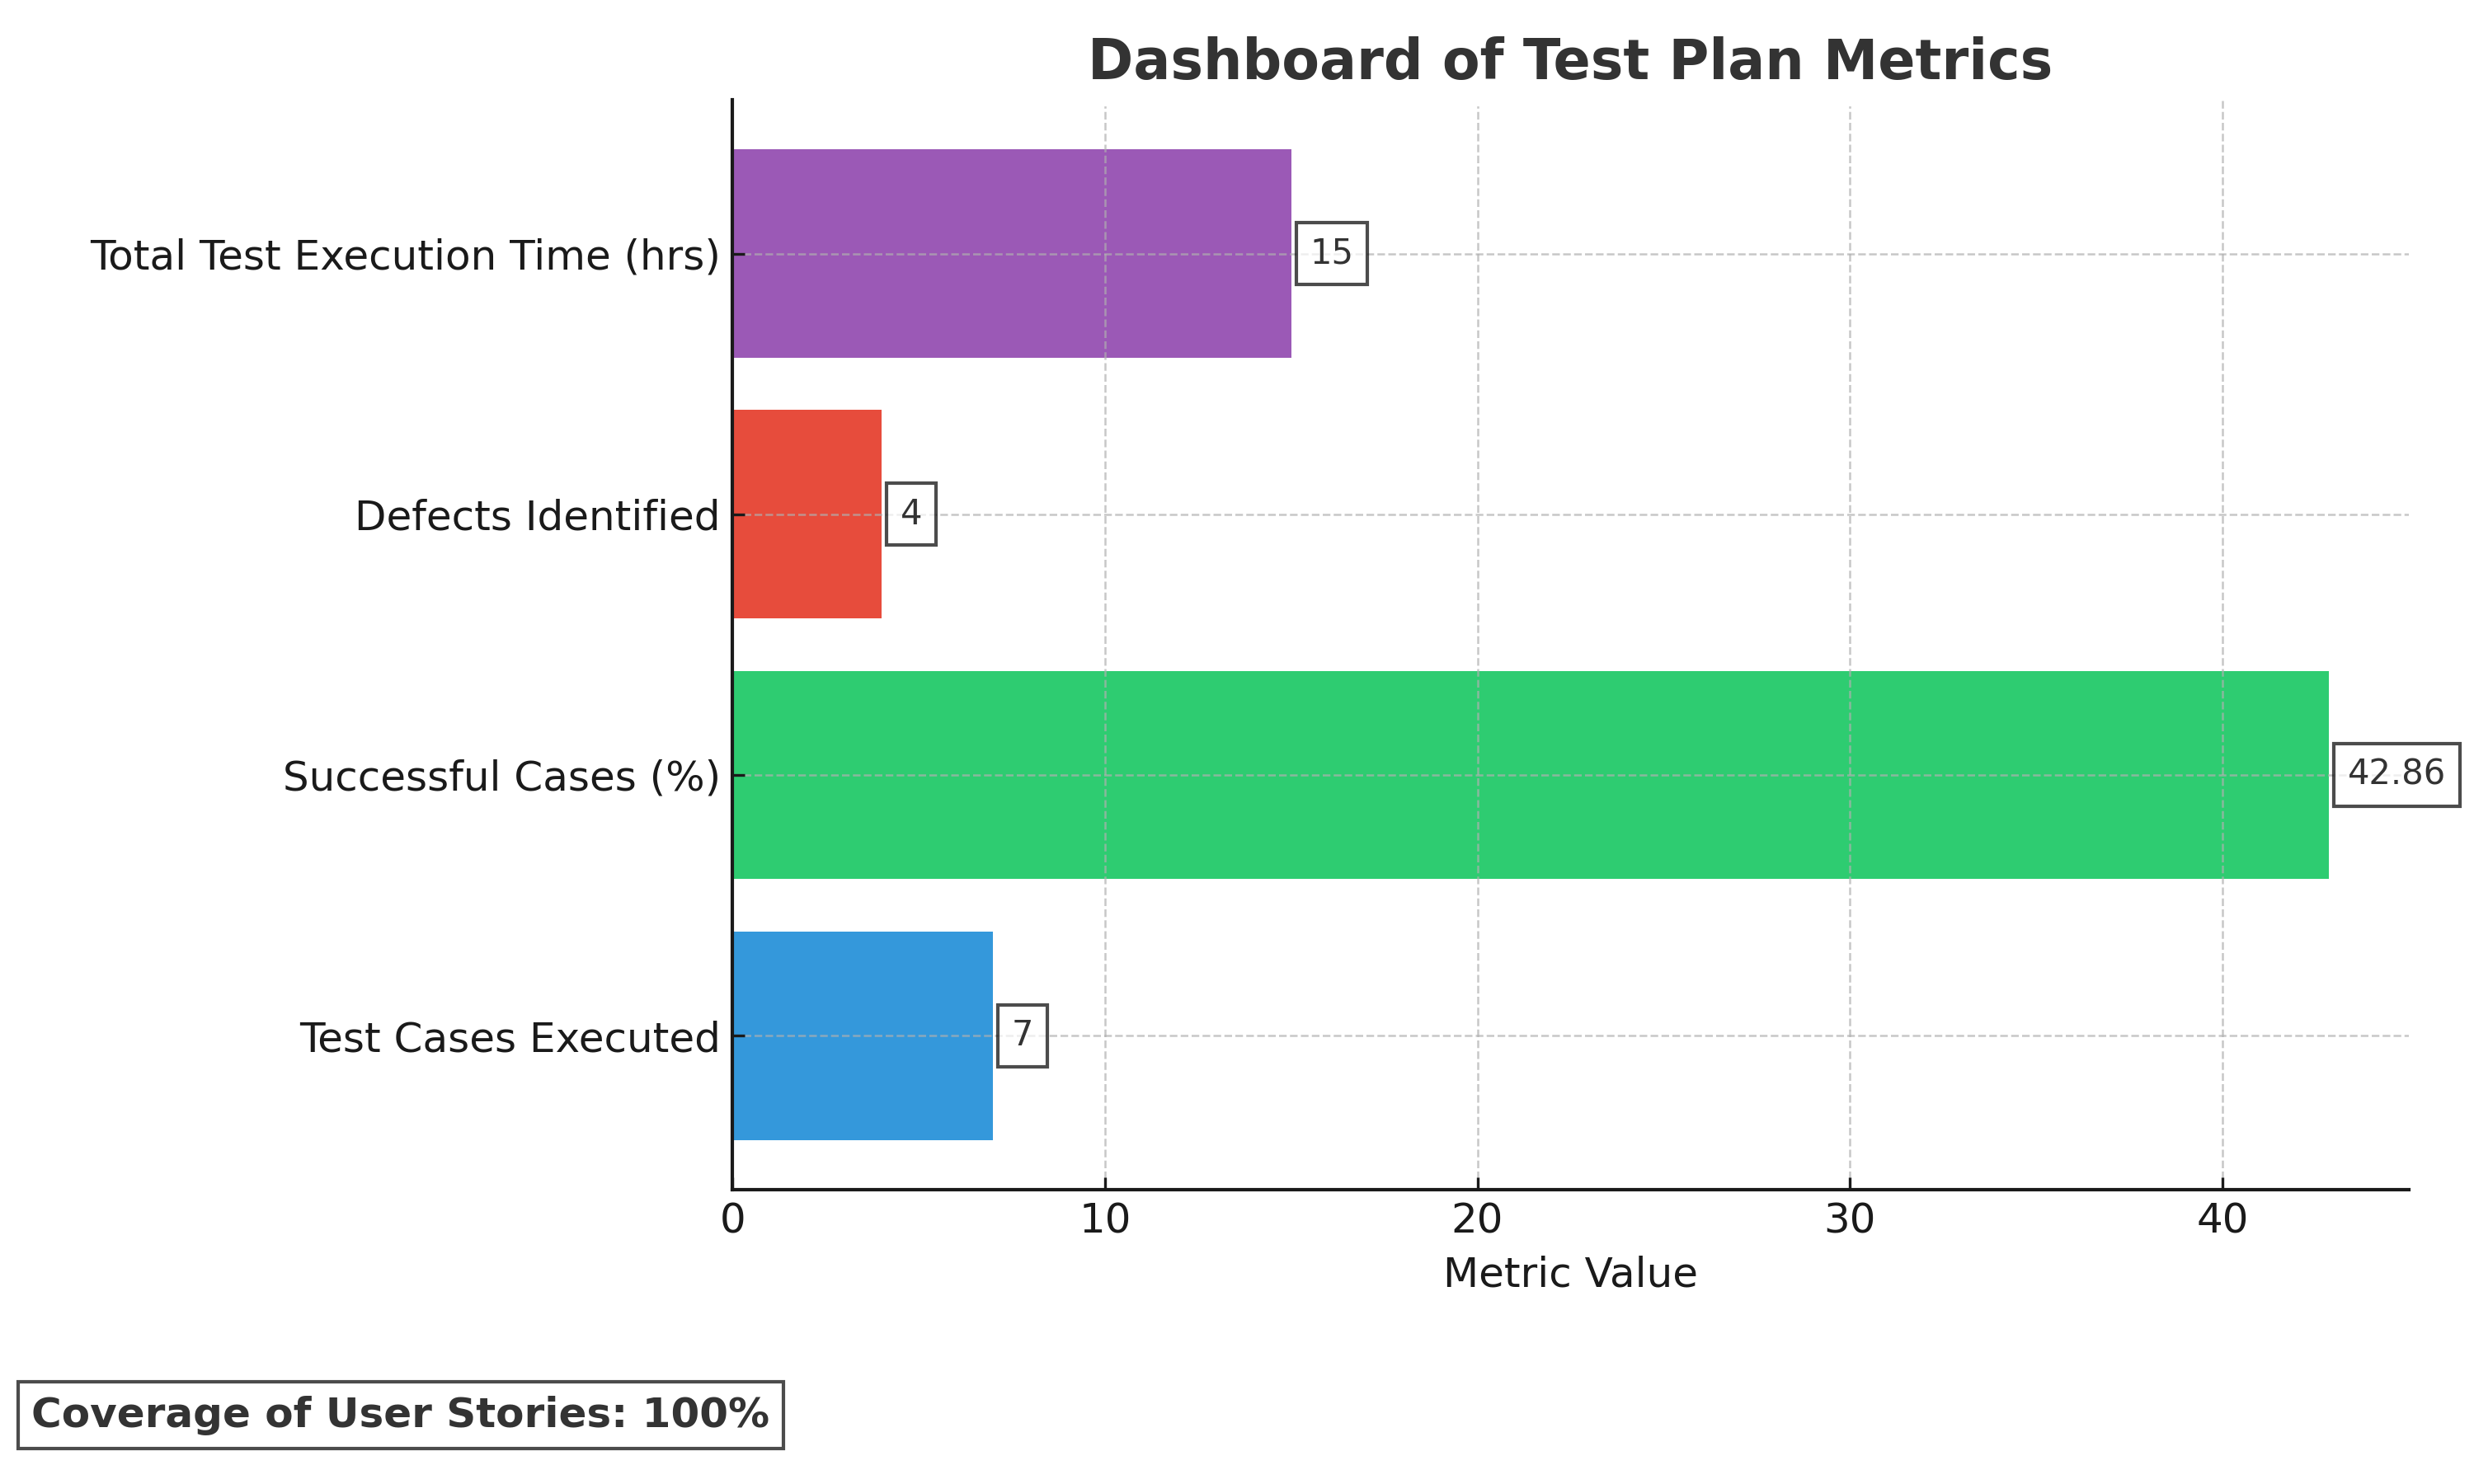
\includegraphics[width=\textwidth]{../imgs/dashboard_test_metrics_white_bg.png}
    \caption{Dashboard de Métricas del Plan de Pruebas}
\end{figure}

\subsection{Resultados Obtenidos en Pruebas de Accesibilidad}

\noindent Las pruebas de accesibilidad realizadas con Axe DevTools revelaron varios problemas de accesibilidad, aunque en general, la cantidad de defectos encontrados no fue excesiva, lo cual es un indicio de que el sistema ya cuenta con una base relativamente sólida en términos de accesibilidad. A continuación, se detalla cada uno de los problemas identificados:

\begin{longtable}{|p{3cm}|p{10cm}|}
    \caption{Reporte de Accesibilidad} \label{tab:reporte_accesibilidad} \\
    \hline
    \multicolumn{2}{|c|}{\textbf{WCAG 2.1 AA}} \\ \hline
    \textbf{Guideline} & \textbf{Descripción de la Violación} \\ \hline
    \endfirsthead

    \hline
    \multicolumn{2}{|c|}{\textbf{WCAG 2.1 AA}} \\ \hline
    \textbf{Guideline} & \textbf{Descripción de la Violación} \\ \hline
    \endhead

    1.1 & Los botones deben tener texto discernible. Se detectaron botones sin texto visible para lectores de pantalla, ni atributos accesibles como `aria-label` o `aria-labelledby`, lo cual impide que los usuarios de tecnologías de asistencia comprendan la función de estos botones. \\ \hline
    1.2 & Los elementos deben tener un contraste de colores suficiente. Se encontraron elementos con un contraste insuficiente entre el texto y el fondo, lo cual no cumple con el estándar mínimo de 4.5:1. Ejemplo: color de primer plano \#17a2b8 en fondo blanco (\#ffffff) con un tamaño de fuente de 16px y grosor en negrita, resultando en un contraste de 3.04:1. Este problema afecta la legibilidad, especialmente para usuarios con discapacidades visuales. \\ \hline
    1.3 & Los elementos de formulario deben tener etiquetas. Algunos campos de entrada no cuentan con etiquetas visibles o accesibles mediante `<label>`, `aria-label`, o `aria-labelledby`, lo cual dificulta la comprensión de estos elementos para los usuarios que dependen de lectores de pantalla. \\ \hline
\end{longtable}

\subsection{Resultados Obtenidos en Pruebas de Usabilidad}

\noindent Las pruebas de usabilidad realizadas permitieron evaluar varios aspectos clave del sistema, como la visibilidad del estado, el control y la libertad del usuario, la consistencia y estándares, entre otros. En general, se detectaron áreas de mejora en términos de consistencia visual, retroalimentación al usuario, y navegación, los cuales se detallan en los resultados adjuntos. Cabe destacar que el sistema cumple con algunos de los principios fundamentales, como la flexibilidad y la visibilidad en varias de sus opciones, lo cual es positivo para la experiencia de usuario.

\noindent Para una descripción completa de los resultados obtenidos en cada ítem evaluado, por favor consulte los detalles (\hyperref[tab:reporte_usabilidad]{en Anexos})


\section{Conclusiones}

\begin{itemize}
    \item \textbf{Evaluación general del sistema:} Los resultados obtenidos en las pruebas indican que el sistema cumple con la mayoría de las funcionalidades requeridas. Sin embargo, se identificaron varias áreas de mejora en términos de validación de datos, usabilidad, accesibilidad y feedback visual al usuario. Estas mejoras son críticas para alcanzar un sistema más robusto y alineado con las necesidades de los usuarios.

    \item \textbf{Validación de datos y manejo de errores:} Se detectaron defectos en la validación de campos obligatorios y numéricos, así como en la notificación de errores en entradas inconsistentes. Estos problemas pueden llevar a errores de entrada, afectando la precisión de los cálculos y la experiencia de usuario. Es recomendable implementar mecanismos de validación más rigurosos y notificaciones específicas para guiar a los usuarios en la corrección de errores.

    \item \textbf{Accesibilidad y usabilidad:} A pesar de cumplir con algunos principios de accesibilidad, se observaron deficiencias en el contraste de colores, la etiquetación de elementos de interfaz y el feedback visual. Esto impacta especialmente a usuarios con discapacidades visuales. La implementación de mejoras en accesibilidad no solo cumpliría con los estándares de WCAG, sino que también mejoraría la experiencia de todos los usuarios.

    \item \textbf{Retroalimentación y consistencia visual:} Las pruebas de usabilidad evidenciaron la falta de consistencia en elementos visuales y retroalimentación insuficiente para algunas interacciones. Se recomienda estandarizar los íconos, colores, y mensajes del sistema, así como ofrecer retroalimentación inmediata para cada acción del usuario. Esto facilitará la navegación y reducirá la curva de aprendizaje del sistema.

    \item \textbf{Gestión de riesgos y defectos persistentes:} Varios defectos identificados en las pruebas de funcionalidad y usabilidad representan riesgos no mitigados que afectan la estabilidad y confiabilidad del sistema. La falta de ajuste automático en situaciones de desbalance entre oferta y demanda, junto con la ausencia de notificaciones para datos inconsistentes, son áreas críticas que requieren atención inmediata para evitar problemas en el uso del sistema en entornos de producción.

    \item \textbf{Recomendaciones para próximas iteraciones de pruebas:} 
    \begin{itemize}
        \item Mejorar el proceso de validación de datos, asegurando que todos los campos requeridos y numéricos tengan validaciones adecuadas y que el sistema emita mensajes de error específicos y comprensibles.
        \item Implementar mejoras en la accesibilidad mediante la optimización de contraste de colores, adición de etiquetas descriptivas para lectores de pantalla y simplificación de la navegación.
        \item Fortalecer el feedback visual, asegurando que el sistema proporcione retroalimentación clara y consistente para todas las acciones del usuario.
        \item Realizar pruebas de usabilidad con usuarios finales para identificar oportunidades adicionales de mejora en la interfaz, especialmente en términos de diseño minimalista y reconocimiento de errores.
    \end{itemize}

    \item \textbf{Conclusión final:} Si bien el sistema cumple con muchos de los requisitos funcionales, las áreas de accesibilidad, usabilidad y manejo de errores necesitan mejoras significativas para que el producto sea verdaderamente accesible y fácil de usar. Se recomienda abordar las áreas mencionadas en futuras iteraciones de desarrollo para optimizar el sistema y mejorar la experiencia del usuario, asegurando que el producto final cumpla con los estándares de calidad esperados.
\end{itemize}


\newpage
\section{\large Anexos}

\subsection{Anexo A: Reporte de Defectos de Usabilidad} \label{tab:reporte_usabilidad}

\begin{longtable}{|>{\raggedright\arraybackslash}p{10cm}|>{\centering\arraybackslash}p{3cm}|}
    \caption{Plantilla de Reporte de Usabilidad} \label{tab:reporte_usabilidad} \\
    \hline
    \textbf{Items} & \textbf{Evaluation} \\ \hline
    
    \textbf{1.- Visibilidad del estado del sistema} & \\ \hline
    ¿Cada parte de la interfaz comienza con un título que describa el contenido de la pantalla? & Conforme \\ \hline
    ¿El diseño de íconos y su estética es consistente en todo el sistema? & Conforme \\ \hline
    Cuando se selecciona un icono que está rodeado de otros iconos, ¿Se distingue claramente el ícono seleccionado? & No Conforme \\ \hline
    Si se utilizan ventanas emergentes (pop-up) para mostrar mensajes de error, ¿Permiten esas ventanas que el usuario visualice el error en la interfaz cuando se despliegan? & No Conforme\\ \hline
    ¿Hay algún tipo de feedback para cada acción u operación? & No Conforme\\ \hline
    Luego de que el usuario completa una acción o serie de acciones, ¿El "feedback" del sistema indica que el siguiente grupo de acciones puede completarse? & No Conforme\\ \hline
    El sistema provee algún tipo de feedback visual en menús o cajas de diálogo que indiquen qué opciones pueden seleccionarse. & Conforme \\ \hline
    El sistema provee algún tipo de feedback visual en menús o cajas de diálogo que indiquen en cuál de las posibles opciones se halla posicionado el cursor. & No Conforme \\ \hline
    Si hay menús o caja de diálogo en donde pueden seleccionarse múltiples opciones, ¿El sistema provee algún tipo de "feedback" visual que indique cuáles son las opciones ya seleccionadas? & No Conforme \\ \hline
    ¿El sitio web entrega información corporativa de la organización? & Conforme \\ \hline
    Si existen demoras mayores a 15 segundos en las respuestas del sistema, ¿El usuario es informado del progreso en la concreción de la respuesta? & No Conforme \\ \hline
    ¿Informa datos relevantes para quien no "navega" (Ej: Horas de atención)? ¿Y para hacer consultas web o no web (Ej: números de teléfono)? & No Conforme \\ \hline
    ¿Los tiempos de respuesta son apropiados para cada tarea? & Conforme \\ \hline
    Tiempo de escritura, movimiento del cursor o selección con el ratón: entre 0,5 y 1,5 milisegundos & Conforme \\ \hline
    Tareas más comunes: 2 a 4 segundos & Conforme \\ \hline
    Tareas complejas: 8 a 12 segundos & Conforme \\ \hline
    No son necesarios altos niveles de concentración y no es requerido retener información: 2 a 15 segundos & No Conforme\\ \hline
    La terminología usada en los menús, ¿Es consistente con el dominio de conocimiento del usuario en relación a la tarea a realizar? & Conforme \\ \hline
    ¿El usuario conoce su ruta de ubicación? & Conforme \\ \hline
    
    \textbf{2.- Relación entre el sistema y el mundo real} & \\ \hline
    ¿Los íconos son concretos y familiares para el usuario? & Conforme \\ \hline
    ¿Los colores seleccionados corresponden a los valores esperados? & No Conforme \\ \hline
    Cuando se ingresan datos en la pantalla, ¿La terminología utilizada para describir la tarea es familiar para los usuarios? & Conforme \\ \hline
    Cuando la pantalla incluye preguntas, ¿El lenguaje de esas preguntas es claro y conciso? & N/A \\ \hline
    Las combinaciones de secuencias de letras o palabras extrañas o poco frecuentes, ¿Se evitan siempre que sea posible? & No Conforme\\ \hline
    El sistema ingresa/elimina de manera automática los signos de pesos o dólar y decimal cuando se insertan valores monetarios. & N/A\\ \hline
    ¿Se utilizan nombres unívocos y descriptivos en todo momento? & No Conforme \\ \hline
    ¿Se hace uso de los rastreadores de progreso? & No Conforme\\ \hline
    Los H1 están optimizados para SEO & No Conforme \\ \hline
    
    \textbf{3.- Control y libertad  por parte del usuario} & \\ \hline
    En sistemas que permitan el uso de ventanas superpuestas ¿Es fácil reacomodar reubicar esas ventanas en la pantalla? & Conforme \\ \hline
    En sistemas que permitan el uso de ventanas superpuestas ¿Es fácil para los usuarios cambiar de una ventana a otra? & Conforme \\ \hline
    Cuándo una tarea efectuada por el usuario se completa ¿el sistema espera alguna señal del usuario antes de procesar la tarea? & Conforme \\ \hline
    ¿Se pregunta al usuario que confime acciones que tendrán consecuencias drásticas, negativas o destructivas? & No Conforme \\ \hline
    ¿Existe una función para "deshacer" al nivel de cada acción simple, cada entrada de datos y cada grupo de acciones completadas? & No Conforme \\ \hline
    ¿Los usuarios pueden cancelar acciones en progreso? & No Conforme \\ \hline
    ¿Los usuarios pueden reducir el tiempo de entrada de datos copiando y modificando datos existentes? & Conforme \\ \hline
    Los menús son anchos (muchos ítems), antes que profundos (muchos niveles) & No Conforme \\ \hline
    Si el sistema posee menús de niveles múltiples ¿Existe algún mecanismo que permita a los usuarios regresar al menú previo? & Conforme \\ \hline
    Los usuarios pueden moverse hacia delante o hacia atrás entre las opciones de campos o cajas de dialogo. & Conforme \\ \hline
    Si el sistema utiliza una interfaz de preguntas y respuestas ¿Pueden los usuarios regresar a la pregunta anterior o saltear hacia delante una pregunta? & N/A \\ \hline
    ¿Los usuarios pueden revertir sus acciones de manera sencilla? & Conforme \\ \hline
    Si el sistema permite a los usuarios revertir sus acciones , ¿Existe un mecanismo que permita "deshacer" varias acciones de manera simultánea?  & No Conforme \\ \hline

    \textbf{4.- Consistencia y estándares} & \\ \hline
    El abuso de letras en mayúscula en la pantalla se ha evitado & No Conforme \\ \hline
    No hay más de 12/20 tipos de íconos & Conforme \\ \hline
    Existe algún elemento visual que identifique la ventana activa & Conforme \\ \hline
    Cada ventana posee un título & Conforme \\ \hline
    ¿Es posible utilizar las barras de desplazamiento horizontal y vertical en cada ventana? & Conforme \\ \hline
    Si una opción de un menú es la de "salir" ¿Esta opción aparece como ultimo ítem en el menú? & No Conforme \\ \hline
    ¿Los títulos de los menús están centrados o justificados a la izquierda? & No Conforme\\ \hline
    Fuentes: hasta tres tipos como máximo & No Conforme\\ \hline
    Hasta cuatro colores (usados ocacionalmente)  & No Conforme \\ \hline
    Sonido: tonos suaves para dispositivos de retroalimentación ocacional y bruscos para condiciones críticas. & N/A\\ \hline
    ¿Se provee una leyenda si los códigos de color son numeros o dificiles de interpretar?  & No Conforme \\ \hline
    Se evitan los pares de colores espectralmente extremos y altamente  cromáticos & No Conforme \\ \hline
    Los azules saturados no se utilizan para texto u otro elemento pequeño. & No Conforme \\ \hline
    La información más importante esta above the fold (la parte del sitio que los usuarios ven primero) & No Conforme \\ \hline
    ¿La estructura de la entrada de datos es consistente entre las diferentes pantallas? & No Conforme \\ \hline

    \textbf{5.- Prevención de errores} & \\ \hline
    ¿Las entradas de datos no son sensibles a mayúsculas siempre que sea posible? & No Conforme \\ \hline
    Las pantallas para entrada de datos y cajas de diálogo indican el número de espacios en caracteres que estan disponibles para un campo & No Conforme \\ \hline
    Los campos en las pantallas de entrada de datos y las cajas de diálogo ¿contienen valores por defecto cuando corresponden? & No Conforme \\ \hline

    \textbf{6.- Reconocer antes que recordar} & \\ \hline
    ¿Las áreas de texto tienen "espacios de respiración" que las rodeen? & No Conforme \\ \hline
    ¿Se ha utilizado el mismo color para agrupar elementos relacionados? & No Conforme \\ \hline
    ¿Existe buen contraste de brillo y de color entre los colores usados para imágines y fondos? & No Conforme \\ \hline
    Los colores suaves, brillantes y saturados se han utilizado para enfatizar datos, mientras que los colores oscuros, opacos y no saturados, han sido usados para des-enfatizar datos? & No Conforme \\ \hline
    ¿Los ítems inactivos en un menú aprecen en gris o están omitidos? & No Conforme \\ \hline

    \textbf{7.- Flexibilidad y eficiencia en el uso} & \\ \hline
    Los usuarios pueden reducir el tiempo de entrada de datos si se les permite copiar y pegar datos existentes. & Conforme \\ \hline
    Si las listas de menú son cortas (siete ítem o menos) ¿Pueden los usuarios seleccionar un ítem moviendo el cursor? & Conforme \\ \hline

    \textbf{8.- Diseño estético y minimalista} & \\ \hline
    Los íconos son visuamente distinguibles de acuerdo a su significado conceptual  & Conforme \\ \hline
    ¿Cada ícono esta resaltado con respecto a su fondo? & Conforme \\ \hline
    Cada pantalla de entrada de datos incluye un título simple, corto, claro y suficientemente distintivo. & No Conforme \\ \hline
    Los títulos de los menús son breves pero lo suficientemente largos como para comunicar su contenido. & No Conforme \\ \hline

    \textbf{9.- Ayuda a los usuarios a reconocer, diagnosticar y recuperarse de los errores} & \\ \hline
    ¿Los sonidos son utilizados para señalar errores? & N/A \\ \hline
    Si se usan mensajes de error con humor ¿Son apropiados y respetuosos para la comunidad de usuarios? & No Conforme\\ \hline
    ¿Los mensajes de error son gramaticalmente correctos? & Conforme \\ \hline
    ¿Los mensajes de error evitan el uso de signos de admiración? & No Conforme\\ \hline
    Los mensajes de error evitan el uso de palabras violentas u hostiles & No Conforme\\ \hline
    Si se detecta un error en un campo de entrada de datos ¿El sistema posiciona el cursor en ese campo o lo resalta de alguna manera? & No Conforme \\ \hline
    ¿Los mensajes de error sugieren la causa del problema que lo has ha ocacionado? & No Conforme \\ \hline
    ¿Los mensajes de error indican que acción debe realizar el usuario para corregir el error correspondiente? & No Conforme \\ \hline

    \textbf{10.- Ayuda y documentación} & \\ \hline
    ¿Las instrucciones en linea se distnguen visualmente?  & No Conforme \\ \hline
    Si las opciones de los menús son ambiguas ¿el sistema provee información aclaratoria adacional cuando un ítem es seleccionado? & No Conforme \\ \hline
    ¿La función de ayuda del menú es visible? (Por ejemplo una tecla etiquetada AYUDA o un menú especial) & No Conforme \\ \hline
    Navegación: la información es facíl de encontrar & Conforme \\ \hline
    ¿La información es exacta, completa y comprensible? ¿La información es relevante? & No Conforme \\ \hline
    Tras haber accedido a la ayuda ¿Pueden los usuarios continuar con su trabajo desde donde ha sido interrumpido? & Conforme \\ \hline
    ¿Es fácil acceder y regresar del sistema de ayuda? & Conforme \\ \hline
\end{longtable}

\end{document}
